% !TeX root = ../../thesis.tex
\chapter{Literature review}\label{ch_anisoIEintro}

\section{Microstructure formation in coatings}
Microstructure here denotes both the morphology on the surface, shape and size of grains and their crystallographic texture.

The experimental investigations of the texture-forming factors in deposits are usually specific for the particular deposition method, like physical vapour deposition (PVD), sputtering or electrodeposition. Despite some obvious differences between the methods, it is natural to expect the textures to be formed by the same mechanisms. These are necessarily altered by the method-specific deposition conditions, thus giving rise to some behaviors which are then considered as standard for that type of deposition. 

For example, the Structure Zone Model (SZM)~\cite{Barna1998} is often used to describe the dependence of microstructure on the relative deposition temperature in PVD and sputtering methods, but not so in electrodeposition. There, rather the Winand diagram~\cite{Winand1992} is used instead, having the axes representing degree of chemical surface inhibition and current density, i.e. deposition rate. Both of these can be perceived as state diagrams, where the individual regions qualitatively indicate the one microstructure/morphology which is most likely to be stable for those deposition conditions. Interestingly, in electrodeposition the crystallographic texture of the coating does not necessarily imply a particular deposit morphology in electrodeposition

Barna~\cite{Barna1998} claims, that the different crystallographic textures observed in PVD or sputter deposition can be correlated to the respective \textit{structure zone}. Specifically, he uses the terms \textit{competitive growth texture} and \textit{restructuration growth texture}, which correspond to the ones where the resulting texture depends on either the anisotropy in growth rate or on the concurrent minimization of surface and grain boundary energy, respectively.

In electrodeposition, the situation is more complicated than in PVD or sputtering by the presence of the double layer on the metal surface and the complex interplay of the electric field and chemical reactions between all the species.  Nevertheless, experimental work largely shows that, as far as three-dimensional nucleation is concerned, the same observations are made in electrocrystallization
and in physical crystallization~\cite{Winand1992}: increasing the deposition rate and/or increasing the inhibition usually results in increased nucleation rate and thus eventually in the reduction in the deposit grain size. .

The inhibition refers to some specific interactions between the deposit and the parent phase. The inhibiting species attaches to low-energy sites where the growth might easily proceed and then the adatoms must find another spot to settle down, having their lifetime before being incorporated into the crystal potentially prolonged and thus increasing the nucleation probability~\cite{Winand1992}. The inhibitor may be a natural constituent of the electrolyte in electrodeposition or simply some impurity. In PVD deposition of aluminium with variable amounts of oxygen, it was observed that increased oxygen amounts reduced the grain size up to nanocrystalline or even amorphous coating of alumina~\cite{Barna1998}.

A separate field of research involves stress in the deposits~\cite{Thornton1989, Thompson1993, Chason2015, Abadias2018}. Both tensile and compressive stress are observed in the deposits depending on the deposition conditions and deposited material. Generally speaking, higher temperatures and lower deposition rates (i.e. deposition closer to thermodynamic equilibrium) lead to behavior, where a compressive stress develops with increasing thickness of the film, but after the deposition stops, the stress either completely or partly relaxes. This is highly dependent on the material too, where materials with higher self-diffusion coefficient (lower melting point) tend to exhibit such behavior~\cite{Chason2002}. On the other hand, high growth rates and low deposition temperatures (i.e. rather off-equilibrium deposition) lead to tensile stresses, which do not relax after the deposition termination. Materials with lower self-diffusion coefficients (higher melting points) are associated with these. Another source of stress can be interactions with the substrate.

Stress can suppress or promote grain growth~\cite{Thompson1993}. It is then natural to consider stress relaxation as another texture-forming process. As was mentioned in the Introduction, the fundamental texture-forming quantities are interfacial energy, surface diffusivity of adatoms, grain boundary mobility and grain boundary and lattice diffusion~\cite{Szpunar1997, Suwas2014}. However, it is the particular state of the material and the deposition conditions, which then drives the deposit to evolve in particular ways.

Thompson~\cite{Thompson1993} developed an abstracted model of columnar microstructure and expressed its total strain and total interface energy as function of thickness. Because the thickness dependence of these energies was different, the model suggested that the texture could be dominated by minimization of interface energy below certain (temperature-dependent) thickness and above it, the texture would be dominated by the strain energy minimization. Especially in the light of the previous paragraph, it is clear that the stress state of a real deposit does not depend only on the deposit thickness. Nevertheless, the idea of having different mechanisms competing over the course of texture/morphology evolution as the film thickness increases is strongly based in experimental observation. Also, the terms \textit{interface-energy minimization texture} or \textit{strain-energy minimization texture} are used in practice~\cite{Alimadadi2016}.

Specifically in electrodeposition, the inhibition in relation to the morphology and texture was studied extensively~\cite{Winand1992}. Amblard~\cite{Amblard1979} determined the particular species responsible for the texture variation in nickel electrodeposits from Watts electrolyte when varying the pH, current density and adding separately a brightening and levelling agents. These species selectively inhibited the metal surface and thus introduced different textures. A more recent study~\cite{BergenstofNielsen1997} reviewed other hypotheses about the possible texture-forming processes in nickel electrodeposition from Watts electrolyte and after transmssion electron microscopy study of one deposit, they concluded that the inhibition was the most likely scenario. 

The same group later proposed~\cite{Rasmussen2001}, that the texture of an electrodeposit could develop from a zone mainly affected by the substrate (epitaxy, chemical reactions), through a zone of mixed control to a zone affected solely by the deposition conditions (selective inhibition, deposition rate). However, in a more recent study~\cite{Alimadadi2016} involving microtexture measurement through thickness of the nickel electrodeposits obtained at different pH and current density, the authors could not confirm the existence of the transition zone as a simple mixture of the substrate- and conditions-affected zones. 

\section{Specific surface and interface energy}
Be there an isothermic isolated thermodynamic system consisting of a block of solid material in a vacuum. When the block is reversibly cleaved, two equal areas $A$ are created on each side of the cleavage, newly facing the vacuum. The total energy change upon cleavage is equal to the reversible work $W$ done on the system. The reversible work thus transforms into \textit{surface energy} (unit \unit{J}) of the cleavage areas $W=2A\sigma$, where the symbol $\sigma$ stands for the \textit{specific surface energy} (unit \unit{J/m^2})~\cite{Milchev2002}. 

Should the system consist of the solid block within a liquid, the specific surface energy would be lower due to interactions between the liquid and solid (e.g. specific interactions of the molecules within the liquid with the surface or double layer formation in case of electrified surface). The same in fact holds for blocks of two different materials joined together by an \textit{interface}, meaning that the \textit{interface energy} will be lower than the sum of the individual surface energies (by \textit{adhesion energy}). The interface is then characterized by \textit{specific interface energy}. Even though some sources strictly distinguish the \textit{interface} to occur between two solid phases and use the word \textit{surface} for the solid in both vacuum or liquid~\cite{Milchev2002}, it as valid to see the \textit{interface} between two dissimilar phases (e.g. solid and liquid) and reserve the term surface energy strictly for the solid in vacuum. This thesis rather sees what separates the liquid from solid as \textit{interface}, but care was taken to be always explicit enough to make it clear what is the particular quantity in question.

The word \textit{specific} in the \textit{specific surface energy} indicates that the quantity is intensive, i.e. relative to the area in this case. However, especially in phase field literature it is rather common to denote the intensive quantity simply by \textit{surface energy} or \textit{interface energy}. These two are often used interchangeably in this thesis.


\section{Anisotropic interface energy}
Let the interface energy $\sigma$ depend on the local orientation of the interface described by its unit normal $\bm{n}$, i.e. $\sigma=\sigma(\bm{n})=\sigma_0 h(\bm{n})$. The function $h(\bm{n})$ is called anisotropy function and $\sigma_0$  is a scaling parameter with dimensions of interface energy. Formal requirements on the anisotropy function can be found e.g. in~\cite{Kobayashi2001}. A very useful formalism for thermodynamic description of these anisotropic interfaces is so-called capillary vector $\bm{\xi}$ (a.k.a. Cahn-Hoffmann vector or $\xi$-vector), defined as~\cite{Hoffman1972,Cahn1974}
\begin{equation}
    \bm{\xi} = \mathrm{grad}(r\sigma(\bm{n}))\,,
\end{equation}
where $r$ is radial distance from origin, which can be also seen as magnitude of scaled normal vector $\bm{r}=r\bm{n}$. Level sets of the scalar function $r\sigma(\bm{n})$ are geometrically similar to the anisotropy function $h(\bm{n})$, which is continuously scaled by the radius $r$.

Capillary vector was introduced and investigated by Hoffman and Cahn in~\cite{Hoffman1972,Cahn1974}, who showed that this formalism is consistent with major laws governing behavior of (anisotropic) interfaces like Gibbs-Thompson equation (relating chemical potential and isotropic surface curvature), Herring's equation (chemical potential on anisotropic curved surface), Wulff shape construction, force balance at multi-junctions and others. 

A defining property of capillary vector is that its component normal to the surface $\xi_\perp$ is in magnitude equal to the local value of the interface energy and the surface-tangent component points in the direction of steepest change in interface energy and is proportional to the change. More specifically  
\begin{align}
    \xi_\perp &= \bm{\xi}\cdot\bm{n}=\sigma(\bm{n}) \\
    \xi_\| &= \left(\frac{\partial \sigma}{\partial \theta}\right)_{max} \,,
\end{align}
where $\theta$ is the angle representing change in orientation of $\bm{n}$ in the direction of maximal angular rate change. The vector can thus be written
\begin{equation}
    \bm{\xi}(\bm{n}) = \sigma(\bm{n})\bm{n} + \left(\frac{\partial \sigma}{\partial \theta}\right)_{max} \bm{t} \,,
\end{equation}
with $\bm{t}$ being unit vector tangent to the surface pointing in the described direction. Useful is expression of capillary vector in spherical coordinates 
\begin{equation}
    \bm{\xi}(\theta,\phi) = \sigma(\theta,\phi)\bm{\hat{r}} + \left(\frac{\partial \sigma}{\partial \theta}\right)\bm{\hat{\theta}} + \frac{1}{\sin(\theta)}\left(\frac{\partial \sigma}{\partial \phi}\right)\bm{\hat{\phi}} \,,
\end{equation}
which is only function of the polar and azimuthal angle $\theta,\phi$, respectively. In 2D in polar coordinates the normal and tangent vector can be written as functions of the interface normal angle $\theta$ as
\begin{equation} \label{eq_xivec_2D}
    \bm{\xi}(\theta) = \sigma(\theta)\begin{bmatrix}
          \cos(\theta)  \\
          \sin(\theta) 
     \end{bmatrix} + \left(\frac{\partial \sigma}{\partial \theta}\right)\begin{bmatrix}
          -\sin(\theta) \\
          \cos(\theta)  
     \end{bmatrix} \,.
\end{equation}

\section{Interface stiffness}
The interface stiffness is the coefficient of the interface curvature in the description of the capillarity contribution to the chemical potential. In curvature-driven interface migration, the interface velocity is proportional to the interface stiffness, mobility and curvature.~\cite{Du2007} The so-called Herring's equation originally published in 1951 and reprinted in~\cite{Herring1999} states the chemical potential of atoms on a curved surface $\mu_{surf}$ due to the capillarity in a point P
\begin{equation}
	\mu_{surf} = V_m\left(\sigma + \frac{\partial^2 \sigma}{\partial n_1^2} \right)\frac{1}{R_1} + V_m\left( \sigma +\frac{\partial^2 \sigma}{\partial n_2^2}\right)\kappa_2
\end{equation}
where $n_1, n_2$ are the orthogonal projections of the variable unit vector $\bm{n}$, on which the surface energy $\sigma(\bm{n})$ depends, onto a plane tangent to the surface at the point in question, the direction axis $1$ being chosen in the direction of the principal curvature $1/R_1$, the y axis in that of $1/R_2$ and $V_m$ is the molar volume ~\cite{Herring1999}. For isotropic interface energy $\sigma$
\begin{equation}
	\mu_{surf} = V_m\sigma(\kappa_1+\kappa_2)
\end{equation}
which means the chemical potential is proportional to mean curvature in the point P.

In 2D, the Herring equation simplifies to 
\begin{equation}
	\mu_{surf} = V_m(\sigma + \sigma''(\theta))\frac{1}{R},
\end{equation}
where a prime indicates differentiation and $\theta$ is angle of the normal to the surface.

The interface stiffness $\hat{\sigma}$ in 2D is the scalar quantity $\hat{\sigma} = \sigma + \sigma''(\theta)$, whereas in 3D it is a 2nd rank tensor (i.e. 2x2 matrix), the diagonal terms of which in principal coordinates are $\left(\sigma + \frac{\partial^2 \sigma}{\partial n_1^2} \right), \left( \sigma +\frac{\partial^2 \sigma}{\partial n_2^2}\right)$~\cite{Trautt2005, Du2007, Abdeljawad2018, Moore2021}.
 
The interface velocity due to capillary forces alone $v_\sigma$ is proportional to the chemical potential and the interface mobility $M$~\cite{Herring1999, Trautt2005, Du2007, Abdeljawad2018, Moore2021}
\begin{equation}
	v_\sigma = M\mu_{surf} \,,
\end{equation}
which is valid in this form for both 2D and 3D. This is the way the capillary driving force moves the surface. As a result, the interface stiffness is the key material property that relates interface curvature to interface thermodynamics and kinetics.~\cite{Du2007}

Interface stiffness tensor in 3D is very difficult to measure~\cite{Du2007}. Efforts were made to determine it from models of the interfaces, like e.g. in~\cite{Du2007}, using molecular dynamics simulations~\cite{Trautt2005,Abdeljawad2018} or phase-field crystal method~\cite{Blixt2022}. An attempt to measure part of the anisotropy in grain boundary in the Pb-Sn system experimentally was carried out in~\cite{Rowenhorst2005}. 

Once the values of the anisotropic interface energy are known in the different directions, the interface stiffness can be computed. In the work~\cite{Olmsted2009}, Olmsted carried out a large number of atomistic calculations to provide the grain boundary energy in Al and Ni (face centered cubic metals). These results were later generalized to any fcc metal using a model with only two input material-specific parameters using MATLAB programme GB5DOF~\cite{Bulatov2014}. This was also used to bring insight in the interface stiffness~\cite{Moore2021}

\section{Wulff shape}
Wulff shape is such a shape, which minimizes the interface energy given a constant volume. In 2D it can be obtained as the inner convex hull of all tangent straight lines to the anisotropy function $h(\theta)$. This can be used to define the Wulff shape $W$ as a set of points $\bm{x}$~\cite{Kobayashi2001, Eggleston2001, Salvalaglio2015}
\begin{equation}
    W = \{ \bm{x}\in\mathbb{R}| \bm{x}\cdot\bm{n}\leq \sigma(\bm{n})\} \,,
\end{equation}
which is a geometrical representation of what was said above - projection of the position vector $\bm{x}$ of a point within the Wulff shape to the interface normal vector $\bm{n}$ must be smaller than the anisotropic interface energy. This defines the inner hull of the tangent lines.

When the heads of capillary vectors for all interface normal angles $\theta$ are connected (having a common starting point in the origin), so-called $\xi$-plot is obtained. It turns out, that the $\xi$-plot coincides with the Wulff shape~\cite{Hoffman1972, Kobayashi2001}. Hence, the expression~\eqref{eq_xivec_2D} can be used to plot the 2D Wulff shape in cartesian coordinates. This is entirely true as long as there are no corners or facets on the Wulff shape, in which cases the use of capillary vecor for Wulff shape plotting must be appropriately modified (see below for details).

In~\cite{Cahn1974} the authors re-state he problem of finding equilibrium shapes of crystals with anisotropic interfaces under general conditions. The shape is found as a solution to equation
\begin{equation} \label{eq_xivec_equilibrium_shape}
    \Delta\Omega_v + \nabla_S\cdot \bm{\xi} = 0 \,,
\end{equation}
where $\Delta\Omega_v$ is the bulk driving force, specifically the difference in grand-canonical potential of the two phases, and $\nabla_S\cdot$ is surface divergence. The surface $\bm{r}$ is seeked, complying with the above equation. A simple trick is used to find the shape of an isolated particle. Surface divergence over the surface itself is simply $\nabla_S\cdot\bm{r}=2$, hence we can write
\begin{align}
    1 = \nabla_S\cdot\bm{r}/2 &= -\nabla_S\cdot\bm{\xi}/\Delta\Omega_v \\
     \nabla_S\cdot(\bm{r} +2\bm{\xi}/\Delta\Omega_v) &=0 \,,
\end{align}
leading to the result
\begin{equation}
    \bm{r} = -\frac{2}{\Delta\Omega_v}\bm{\xi} \,.
\end{equation}

This is why the $\xi$-plot coincides with the Wulff shape.

Two different types of singularities may occur in Wulff shapes, which must be treated in a specific way: corners and facets~\cite{Kobayashi2001, Fleck2011}. 

Corners represent a discontinuity of normal angle along the Wulff shape perimeter. They occur when the anisotropy of the interface energy is such, that interface stiffness gets negative for some normal angles $\theta_f$. These angles are called forbidden, because they are thermodynamically unstable. For this reason, they are not present on the Wulff shape. Additionally, there are normal angles $\theta$ which are thermmodynamically stable but are not present on the Wulff shape. The latter ones correspond to angles, where the inverse interface energy $1/\sigma(\theta)$ is non-convex but still have positive interface stiffness. All forbidden angles fall into this non-convex region. By replacing the non-convex part of this function by straight lines a regularized inverse anisotropy function $1/\bar{\sigma}(\theta)$ is obtained. Wulff shape corresponding to the regularized anisotropy function $\bar{\sigma}(\theta)$ does not contain the "ears" behind the corners. The interface stiffness of both the allowed and forbidden angles which form the "ears" were thus set to zero.

The facets occur under angles where there are cusps in the anisotropy function. In a faceted shape, nearly all orientations except for a couple of points are allowed and the $\xi$-plot consists only of those. How to technically extend the equations~\eqref{eq_xivec_2D} so that a full faceted shape is drawn is described e.g. in~\cite{Kobayashi2001}. In practical simulations, this can be solved by replacing the nisotorpy function by such, whichis continuous, but closely approximates the cusped function, see e.g. \cite{Debierre2003}.

\section{Force balance and stability in triple junction} \label{sec_intro_trijun_forcebalance_stability}
A triple junction in 2D is simply a point and a force balance between the three meeting interfaces is achieved if the capillary vectors of the three interfaces sum to zero, i.e.~\cite{Hoffman1972}
\begin{equation} \label{eq_trijun_forcebalance_sum_xivec}
    \bm{\xi}_{12}+\bm{\xi}_{23}+\bm{\xi}_{13}=0 \,.
\end{equation}
This is equivalent to so-called Herring relations which were published in 1951~\cite{Herring1999} and were re-derived by Marks~\cite{Marks2012}
\begin{equation} \label{eq_force_balance_3jun_aniso}
	\sum_{i=1}^3 \left[ \sigma_i(\vartheta_i)\hat{\bm{t}}_i +\frac{\mathrm{d} \sigma_i}{\mathrm{d} \vartheta_i}\hat{\bm{n}}_i \right] = 0 \,,
\end{equation}
where the subscripts now denote interfaces numbered from 1 to 3. $\vartheta_1,\vartheta_2,\vartheta_3$ are angles under which the tangent of each interface is oriented (all with respect to x axis, see the Figure~\ref{fig_Marks2012_sketch_trijun}), the anisotropic interface energies are $\sigma_i(\vartheta_i)$. The triple junction configuration is defined by the triplet of the angles $\vartheta_i$.
\begin{figure}
	\centering
	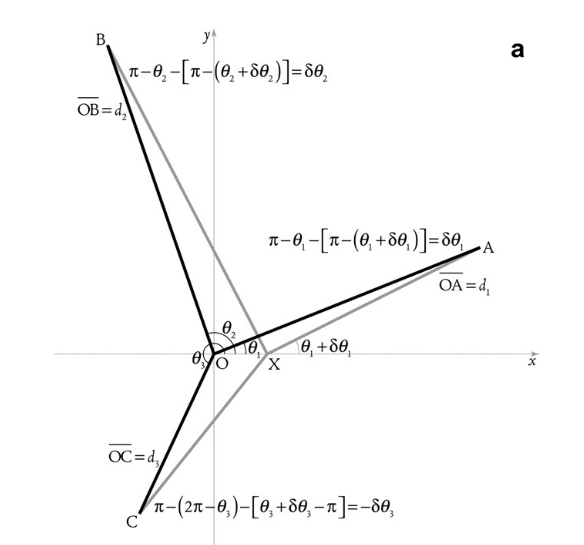
\includegraphics[width=0.6\textwidth]{Marks2021_sketch_trijunction_stability.png}
	\caption{Illustration of a triple junction in 2D taken from~\cite{Marks2012}. Infinitesimal translation in x direction and the corresponding change in the triple junction configuration is illustrated. In the figure the tangent angles of  the individual interfaces are denoted $\theta_i$, whereas in the text they are written as $\vartheta_i$.}
	\label{fig_Marks2012_sketch_trijun}
\end{figure}
However, it was pointed out, that the above equivalent conditions are only \textit{necessary} for the triple junction configuration to be stable, i.e. it does not guarantee the configuration stability. Validity of~\eqref{eq_force_balance_3jun_aniso} assures a stationary point in Gibbs free energy, but in order to have a stable configuration, the energy must be in local minimum. To confirm that, second derivatives of Gibbs free energy with respect to angles $\vartheta_1,\vartheta_2,\vartheta_3$ must be assessed, giving rise to the following two conditions (both of which must hold in stable configuration)
\begin{align} \label{eq_3jun_aniso_stabcond1}
    0 <& \sum_{i=1}^3 \left[ \frac{\mathrm{d}^2 \sigma_i}{\mathrm{d} \vartheta_i^2} + \sigma_i(\vartheta_i) \right]\frac{\sin^2(\vartheta_i)}{d_i} \\  \label{eq_3jun_aniso_stabcond2}
    0 <& \left[ \frac{\mathrm{d}^2 \sigma_1}{\mathrm{d} \vartheta_1^2} + \sigma_1(\vartheta_1) \right]\left[ \frac{\mathrm{d}^2 \sigma_2}{\mathrm{d} \vartheta_2^2} + \sigma_2(\vartheta_2) \right] \frac{\sin^2(\vartheta_1-\vartheta_2)}{d_1d_2} +    \\
     &\quad +\left[ \frac{\mathrm{d}^2 \sigma_2}{\mathrm{d} \vartheta_2^2} + \sigma_2(\vartheta_2) \right]\left[ \frac{\mathrm{d}^2 \sigma_3}{\mathrm{d} \vartheta_3^2} +  \sigma_3(\vartheta_3) \right] \frac{\sin^2(\vartheta_2-\vartheta_3)}{d_2d_3} + \nonumber \\
     &\quad + \left[ \frac{\mathrm{d}^2 \sigma_1}{\mathrm{d} \vartheta_1^2} + \sigma_1(\vartheta_1) \right]\left[ \frac{\mathrm{d}^2 \sigma_3}{\mathrm{d} \vartheta_3^2} + \sigma_3(\vartheta_3) \right]  \frac{\sin^2(\vartheta_3-\vartheta_1)}{d_3d_1} \nonumber \,,
\end{align}
where $d_i$ are lengths from the triple junctions to anchor points, which are not relevant for the current work. Each term in the brackets is interface stiffness of the respective interface.

If the second condition is equal to 0, these conditions are not conclusive, i.e. it is not possible to assess the nature of the stationary point (higher-order derivatives are needed then). 

The assessment of stability of triple junction configuration is an important part of discussion of an equilibrium shape of a particle with anisotropic interface energy on a substrate plane, as will be shown in Chapter~\ref{ch_paper2}.

\section{Equilibrium shapes of a particle with anisotropic interface energy on a planar substrate}
This problem has attracted considerable attention since it is of high practical importance, especially in applications like nucleation~\cite{Bormashenko2021}, preparation of functional deposits for electrochemical catalysis~\cite{Tian2007} or in solid-state dewetting~\cite{PierreLuis2016, Bao2017}. The classical solution to the problem is by Kaischew for crystalline anisotropy with faceted shape~\cite{Kaischew1951} (cited by Milchev in~\cite{Milchev2002} but the original paper was not found) and by Winterbottom \cite{Winterbottom1967} (interface energy as continuous function). Here it is demonstrated using the capillary vector formalism, but the described procedure in its result follows the so-called Winterbottom construction. 

In the following, only 2D cross section is discussed. See the Figure~\ref{fig_winterbottom_explained_intro} for illustration.
\begin{figure}
	\centering
	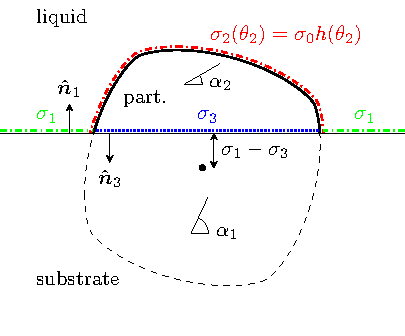
\includegraphics[page=1,width=0.6\textwidth]{sketches_intro.pdf}
	\caption{Illustration of the Winterbottom construction. The symbols $\sigma_1, \sigma_2(\theta), \sigma_3$ denote the interface energiees of the respective interfaces, $\sigma_0$ is the scaling interface energy.  $\alpha_1$ is the orientation of the substrate, $\alpha_2$ of the substrate.}
	\label{fig_winterbottom_explained_intro}
\end{figure}
 It is assumed that the particle-substrate interface (denoted here with index 1) is linear with the substrate-parent phase (index 3), but with anti-parallel normal vector. Let the substrate plane be parallel with x axis. The particle-parent phase interface is denoted by index 2. The normal vectors of the respective interfaces in the contact point are $\hat{\bm{n}}_1=(0,1)^{\mathrm{T}}$, $\hat{\bm{n}}_3=(0,-1)^{\mathrm{T}}$ and $\hat{\bm{n}}_2$ is to be found from~\eqref{eq_trijun_forcebalance_sum_xivec}. Apparently, with the interfaces 1 and 3 fixed at orientations $\theta_1=\pi/2$ and $\theta_3=-\pi/2$, the force balance can be reduced to single equation, when the particle-parent phase capillary vector $\bm{\xi}_2$ is projected to the surface normal $\hat{\bm{n}}_S=\hat{\bm{n}}_3$. But that is merely the y-component of the capillary vector. The force balance can thus be written as
\begin{equation}\label{eq_youngs_eq_aniso}
    \sigma_{3}(\pi/2)-\sigma_1(-\pi/2)  
      = \sigma_2(\theta_2)\sin(\theta_2) + \sigma_2'(\theta_2)\cos(\theta_2) \,.
\end{equation}

Geometric interpretation of this equation is that the force equilibrium in the triple junction is achieved when normal angle $\theta_2$ of the particle-parent phase interface in the triple junction is that one, which has the y coordinate of the Wulff shape equal to the difference $\sigma_{3}(\pi/2)-\sigma_1(-\pi/2) $. The equilibrium shape of anisotropic particle on a substrate is thus that of an isolated particle but truncated at a position, which derives from the force balance in the triple junction. The truncated part of isolated particle counts, which is above the truncating line.

When all the three interfaces are isotropic, the well known Young's equation is obtained
\begin{align}
    \sigma_3-\sigma_1 &= \sigma_2\sin(\theta_2) \\
        &= \sigma_2\cos(\vartheta_2)
    \,,
\end{align}
where in the second equation it was used that $\vartheta_2=\theta_2-\pi/2$.

%Let's assume the anisotropy of the particle-parent phase interface $\sigma_2(\theta_2)=\sigma_2^0h(\theta_2)$. Then the wetting parameter $\Gamma$ is defined
%\begin{equation}
%    \Gamma = \frac{\sigma_{3}(\pi/2)-\sigma_1(-\pi/2) }{\sigma_2^0} \,,
%\end{equation}
%which is the vertical offset of the horizontal truncating line relative to center of the equilibrium shape of unit radius. Apparently, when $\Gamma > 0$, the line is above the Wulff shape center (the shape is submerged below the line) and there is such value of $\Gamma$, when the line is merely a tangent. That corresponds to the case of complete wetting and the contact angle is 0. For isotropic interface energy that occurs for $\Gamma=1$.
%
%On the other hand, when $\Gamma < 0$, the truncating line goes below the center (the shape is emerged above the line). There is such value of $\Gamma$ corresponding to complete non-wetting (with isotropic interface energy that is $\Gamma=-1$).

%\section{Stability of the equilibrium shape}\label{sec_fund_anisoIE_trijun_stability}
%Previous section showed derivation of the 2D equilibrium shape of anisotropic particle on a substrate from the triple junction force balance. However, as explained in~\ref{sec_intro_trijun_forcebalance_stability}, the stability of the solution should be assessed as well. The additional conditions~\eqref{eq_3jun_aniso_stabcond1}, \eqref{eq_3jun_aniso_stabcond2} can be re-written as
%\begin{align}
%    0 &< \Sigma_1 s_1 + \Sigma_2 s_2 + \Sigma_3 s_3 \\
%    0 &< \Sigma_1\Sigma_2 S_{12} + \Sigma_2\Sigma_3 S_{23} + \Sigma_1\Sigma_3 S_{13} \,,
%\end{align}
%where $\Sigma_i = \mathrm{d}^2 \sigma_i/\mathrm{d} \vartheta_i^2 + \sigma_i(\vartheta_i)$ are the respective interface stiffnesses, $s_i = \sin^2(\vartheta_i)/d_i$, $S_{ij} = \sin^2(\vartheta_i-\vartheta_j)/d_i d_j$. Given $\vartheta_1=0$ and $\vartheta_3=\pi$, it follows that $s_1=s_3=0$ and also that $S_{13}=0$. Note also that $s_2>0$ and $S_{12}=S_{23}=S=\sin^2(\vartheta_2)/d^2>0$ (assuming that $d_1=d_2=d_3$). The conditions are thus simplified to
%\begin{align}
%    0 &< \Sigma_2  \label{eq_3jun_stabcond_onplane1}\\
%    0 &< \Sigma_1\Sigma_2 + \Sigma_2\Sigma_3 \,,  
%\end{align}
%where only the interface stiffnesses matter. Using the first equation, the second may further be simplified
%\begin{equation}
%    0< \Sigma_1 + \Sigma_3 \,. \label{eq_3jun_stabcond_onplane2}
%\end{equation}
%The condition~\eqref{eq_3jun_stabcond_onplane1} implies, that the particle-parent phase interface must be oriented under allowed angle in the contact point. That is fulfilled automatically by the truncated Wulff shape solution, because it contains only the allowed angles. 
%
%The condition~\eqref{eq_3jun_stabcond_onplane2} is surely fulfilled when both interfaces 1 and 3 have positive interface stiffness in their orientations. That holds automatically, when the Wulff shapes of the interfaces 1 and 3 do not contain any corners. When both of them do contain corners, it means that there are normal angles where the interface stiffness is negative. Apparently, in such situation, the condition~~\eqref{eq_3jun_stabcond_onplane2} may be violated.

\section{Nucleation fundamentals}
Great majority of phase transformations in metals occurs by nucleation and growth~\cite{Porter2009}. Nucleation is the physical process in which tiny crystals or clusters of a new phase $\mathit{2}$ appear at certain sites within the matrix of a metastable parent phase $\mathit{1}$. Once formed, these nuclei can grow on the expense of $\mathit{1}$. The nucleation rate and nuclei spatial distribution strongly affect the resulting microstructure. The above described process corresponds to homogeneous nucleation. Heterogeneous nucleation, on the other hand, involves one phase more, denoted $\mathit{3}$, on the surface of which the nucleus appears. 

Heterogeneous nucleation is closely related to film deposition. There here are three different types of film growth (termed Volmer-Weber, Frank Van der Merve and Stranski-Krastanov), which are based on two growth mechanisms, termed simply 2D and 3D nucleation. In the 3D nucleation, nuclei appear on the surface of the support as localized 3D clusters and further grow in all directions. In 2D nucleation, monoatomic layers are successively deposited on top of the surface. Volmer-Weber type of growth occurs via the 3D nucleation mechanism, the Frank Van der Merve type via the 2D nucleation and Stranski-Krastanov starts with 2D nucleation but then switches to 3D nucleation. The factor deciding the nucleation mechanism  are the wetting conditions, as will be described farther below. 

The Classical Nucleation Theory poses several fundamental assumptions. In the first place, it assumes that the nuclei are large enough to have defined volume and surface, i.e. that they consist of such number of atoms that is not inadequate to assume continuum-like properties. With nuclei consisting of only a few atoms, these and the derived quantities (e.g. specific surface energy) cannot be defined. Additionally, it assumes that the creation of a nucleus is a instantaneous process, where the necessary number of thermally vibrating atoms occur mutually close enough to overcame the critical nucleation barrier and became a stable growing nucleus. 

"It is worth reminding that, for example, a silver sphere of a radius of only three atomic diameters already contains 106 silver atoms ($d_{\mathrm{Ag}} = \qty{0.252}{nm}$). Cluster sizes of this order are sometimes considered as a lowest limit of the classical nucleation theory validity."~\cite{Milchev2008} The above assumptions seem to be contradictory to some extent, because when imagining thermally fluctuating atoms, it is hard to imagine that \textit{at least} hundreds of atoms would collide at the same time near a single point and instantaneously thus overcame the nucleation barrier.

%During nucleation, the bulk atoms in the parent phase $\mathit{1}$ must locally redistribute and assemble a cluster of phase $\mathit{2}$, which is associated with a new $\mathit{1}$-$\mathit{2}$ interface formation (and in the case of heterogeneous nucleation also new $\mathit{2}$-$\mathit{3}$ interface replacing the former $\mathit{1}$-$\mathit{3}$). In the nucleation site at the instant of nucleation, there must be enough energy to "pay" for the new interface creation. The energy comes from a) reduction in the bulk free energy due to the $\mathit{1}$-$\mathit{2}$ phase transition and from b) thermal fluctuations. The reduction in the bulk free energy is given by the magnitude of driving force to transform from $\mathit{1}$ to $\mathit{2}$ (called undercooling in solidification and supersaturation in general) and by the nucleus volume. Due to thermal fluctuations, the atoms may locally cluster together and if the cluster has larger than critical volume $V_c$, the created interface is stable, i.e. the system energy will be decreased by further nucleus growth. On the other hand, a subcritical cluster will lower the system energy when dissolved.

Because nucleation is a thermally activated process, the probability $P$ of finding the nucleus at a certain spot follows the Arrhenius relation
\begin{equation}
    P \approx \exp\left(-\frac{\Delta G_c^*}{RT}\right) \,,
\end{equation}
where $R$ is the universal gas constant, $T$ absolute temperature and $\Delta G_c^*$ is a \textit{critical nucleation barrier}, which is to be overcome by the thermal fluctuations in order to form a stable nucleus. Nucleus with the critical volume $V_c$ is metastable. The nucleation barrier $\Delta G_c^*$ is the \textit{nucleation work} [Milchev2002], the maximal positive change in Gibbs free energy associated with the nucleus insertion.

% There is homogeneous and heterogeneous nucleation, the homogeneous proceeding exactly as described above and the heterogeneous one involving foreign substrates on which the nucleation barrier is lower. For this reason the heterogeneous nucleation is much more common. 

Shape of the nucleus is strongly determined by the interface energy anisotropy. More specifically, shape of the critical nucleus is such, which minimizes the interface energy, because any other shape would give rise to larger surface energy contribution. The equilibrium shape with isotropic interface energy is a sphere, with an anisotropic one it is a Wulff shape.


% These equilibrium shapes are called Wulff shapes when the interface energy is anisotropic. Equilibrium shape of interface with isotropic interface energy is a sphere.
    \subsection{Nucleation with isotropic interface energy}
        \subsubsection{Homogeneous nucleation}
        Let the difference of Gibbs free energies per unit volume in phases $\mathit{1}$ and $\mathit{2}$ be $\Delta G_v=G_v^\mathit{1}-G_v^\mathit{2}$ and the interface energy $\mathit{1}$-$\mathit{2}$ be $\sigma$. The equilibrium shape is a sphere with radius $R$, surface area $A=4\pi R^2$ and volume $V_{hom}=(4/3)\pi R^3$. The change in Gibbs free energy $\Delta G_{hom}$ is
        \begin{align}
            \Delta G_{hom} &= -\Delta G_v V_{hom} + \sigma A  \\
                &= \frac{4}{3}\pi(-\Delta G_v R^3 + 3\sigma R^2)\,, \label{eq_DG_homog_nucl}
        \end{align}
        and was visualized in Figure~\ref{fig_nucl_barrier}a. From~\eqref{eq_DG_homog_nucl} the expression for the critical radius $R_c$ is found as stationary point $\mathrm{d}(\Delta G_{hom})/\mathrm{d}R=0$, giving the classical result
        \begin{equation} \label{eq_crit_radius}
            R_c = \frac{2\sigma}{\Delta G_v}
        \end{equation}
        and the nucleation barrier is the energy difference value $\Delta G_{hom}(R_c)$ (as can be seen in Figure~\ref{fig_nucl_barrier}a)
        \begin{align}
            \Delta G_{hom}(R_c) = \Delta G_c^* &= \frac{4}{3}\pi\frac{4\sigma^3}{\Delta G_v^2}    \\
                &= \hat{V}_{hom}\frac{4\sigma^3}{\Delta G_v^2} \,,\label{eq_crit_nucl_barrier_hom_iso}
        \end{align}
        where in the second line there was introduced a non-dimensional volume of homogeneous nucleus $\hat{V}_{hom}=V/R^3$.
        
        \begin{figure}
            \centering
            \includegraphics[page=4,width=0.45\textwidth]{sketches_intro.pdf}
            %
            \includegraphics[page=3,width=0.45\textwidth]{sketches_intro.pdf}
            \caption{Bulk (blue) and interface (red) energy contributions to the Gibbs free energy change $\Delta G$ (black) upon nucleus insertion as function of nucleus radius $R/R_c$. Nucleation barrier $\Delta G_c^*$ indicated. In a) as applicable to 3D geometry, in b) as to 2D geometry (see text for details).}
            \label{fig_nucl_barrier}
        \end{figure}
        
        \subsubsection{Heterogeneous nucleation}
        In Figure~\ref{fig_isotropic_wetting} there is illustrated a 2D section through a hemispherical cap on a plane. The three different phases or grains are $\mathit{1}$, $\mathit{2}$ and $\mathit{3}$. Interfaces $\mathit{1}$-$\mathit{3}$ and $\mathit{2}$-$\mathit{3}$ form the substrate plane and are assumed to be immobile. The equilibrium angle $\alpha$ must establish a balance of the tractions due to surface energies of the three distinct interfaces. When the three tractions are projected to the substrate plane, the Young's equation is obtained
        % From equation~\ref{eq_general_trijunction_force_balance} it can be deduced that the force balance in triple junctions of interfaces with isotropic interface energies must satisfy 
        \begin{equation}
            \sigma_{1,3} = \sigma_{2,3} + \sigma_{1,2}\cos(\alpha) \,,
        \end{equation}
        which allows to find the wetting angle $\alpha$ 
        \begin{equation}
            \alpha = \mathrm{acos}\left(\frac{\sigma_{2,3}-\sigma_{1,3}}{\sigma_{1,2}}\right) \,.
        \end{equation}
        The distance of the sphere center to the substrate plane is $R\cos(\alpha)$, which implies
        \begin{equation}
            \Gamma = \cos(\alpha) = \frac{\sigma_{2,3}-\sigma_{1,3}}{\sigma_{1,2}} \,.
        \end{equation}
        
        \begin{figure}
            \centering
            \includegraphics[page=2,width=0.45\textwidth]{sketches_intro.pdf}
            \caption{Heterogeneous nucleation with isotropic interface energy. Force balance in the contact point during surface of $\mathit{3}$ wetting by a nucleus of $\mathit{2}$ emerging from $\mathit{1}$. Nucleus radius $R$ and equilibrium shape center indicated.}
            \label{fig_isotropic_wetting}
        \end{figure}
        
        Upon the nucleus $\mathit{2}$ insertion, the change in Gibbs free energy is
        \begin{align}
            \Delta G_{het} &= -\Delta G_v V_{het} + (\sigma_{2,3}-\sigma_{1,3})A_{2,3} + \sigma_{1,2}A_{1,2} \\
                &= \frac{4}{3}\pi(-\Delta G_v R^3 + 3\sigma R^2) S(\theta) \,, \label{eq_DG_heterog_nucl}
        \end{align}
        where $S(\theta)=(2+\cos\theta)(1-\cos\theta)^2/4$ is the so-called shape factor. The second equation was obtained by using the expressions for the spherical cap volume\footnote{$V_{het}=\pi R^3(2+\cos\theta)(1-\cos\theta)^2/3$}, area\footnote{$A_{1,2}=2\pi R^2(1-\cos\theta)$} and with $A_{2,3}$ being a disc\footnote{$A_{2,3}=\pi(R\sin\theta)^2$}. Two features of~\eqref{eq_DG_heterog_nucl} are to be noted. First, the heterogeneous $\Delta G_{het}$ is equal as in \eqref{eq_DG_homog_nucl} except for $S(\theta)$, and second, the $S(\theta)=V_{het}/(\frac{4}{3}\pi R^3)=V_{het}/V_{hom}$. The shape factor is thus the ratio of the equilibrium volumes of the heterogeneous and homogeneous nuclei of the same interface energy $\sigma_{1,2}$.
        
        Because the $R$-dependence in $\Delta G_{het}(R)$ is equal as in $\Delta G_{hom}(R)$, the critical radius is as in~\eqref{eq_crit_radius}, hence the critical nucleation barrier is 
        \begin{align}
            (\Delta G^*_c)_{het} &= \hat{V}_{hom}S(\theta)\frac{4\sigma^2}{\Delta G_v} \\
                &= (\Delta G^*_c)_{hom}S(\theta)
        \end{align}
            
        Shape factor $S(\theta)$ is thus not only ratio of the equilibrium nuclei volumes, but also of the nucleation barriers. The shape factor is always $0\leq S(\theta)\leq1$. The balance of forces along the contact point of the three phases determines wetting of the surface by the nucleus $\mathit{2}$ which in turn decides about the shape factor and thus the nucleation barrierand also the nucleation mechanism. 
        
        Should the wetting parameter $\Gamma$ be close to or larger than 1, then (nearly) nothing remains of the nucleus \textit{above} the support plane, the shape factor is (nearly) $S=0$ and the 2D nucleation occurs. 
    
    \subsection{Nucleation with anisotropic interface energy}
    When the $\mathit{1}$-$\mathit{2}$ interface energy is anisotropic, the mathematical formalism gets more complicated, but the underlying principles are identical with those in the isotropic case. The Gibbs free energy change is again due to competition between the volumetric and interface energy contributions, but now the interface energy is a function of the interface normal $\bm{n}$, i.e. $\sigma=\sigma(\bm{n})=\sigma_0f(\bm{n})$, with $\sigma_0$ being a scalar and $f(\bm{n})$ an anisotropy function. The nucleus volume is $V_{hom}^{ani}$ and its interface with parent phase is a parameteric surface $\mathcal{S}$. Due to the anisotropy, the interface energy contribution is obtained as a surface integral of $\sigma(\bm{n})$ over $\mathcal{S}$, giving (in homogeneous nucleation) the Gibbs free energy difference
    \begin{equation}
        \Delta G_{hom}^{ani} = -\Delta G_v V_{hom}^{ani} + \int_{\mathcal{S}}\sigma(\bm{n}) \mathrm{d}A \,.
    \end{equation}
    In [Mariaus2010] it was shown, how this can be worked out using the Cahn-Hoffmann $\xi$-vector formalism to reach the familiar expression
    \begin{equation} \label{eq_DG_hom_aniso}
        \Delta G_{hom}^{ani} = (-\Delta G_v X_0^3 + 3\sigma_0 X_0^2)\hat{V}_{hom}^{ani} \,.
    \end{equation}
    where $X_0$ is a scaling parameter for the nucleus size and $\hat{V}_{hom}^{ani}$ the non-dimensional volume $\hat{V}_{hom}^{ani}=V_{hom}^{ani}/X_0^3$.
    As can be seen, the formulas for isotropic critical radius~\eqref{eq_crit_radius} and critical nucleation barrier~\eqref{eq_crit_nucl_barrier_hom_iso} can be generalized for the anisotropic case as
    \begin{equation}
        X_c=\frac{2\sigma_0}{\Delta G_v}
    \end{equation}
    and
    \begin{equation}
        (\Delta G^*_c)_{hom}^{ani} = \hat{V}_{hom}^{ani}\frac{4\sigma_0^2}{\Delta G_v} \,.
    \end{equation}
    
    Also the anisotropic heterogeneous nucleation shows many similarities to the isotropic case. Already Cahn [Cahn,1974] showed, that when the contact line of the substrate and particle is a closed planar curve, the equilibrium heterogeneous nucleus is obtained by truncation of the Wulff shape (in the isotropic case a sphere was truncated). The wetting conditions develop from the force balance along the contact line. That decides how the Wulff shape should be truncated. The force balance includes some extra terms compared to the isotropic case, which will be discussed in the next section. Sketch of the problem is in 
    
    \begin{figure}
        \centering
        \includegraphics[page=7,width=0.45\textwidth]{sketches_intro.pdf}
        \caption{Anisotorpic nucleus of phase $\mathit{2}$ oriented under direction $\bm{n}_\mathit{2}$ wetting the supporting plane $\mathit{3}$. Generalized radius $X_0$ and center shift indicated.}
        \label{fig:my_label}
    \end{figure}
    
    The shape factor $S(\Gamma,\bm{n}_\beta)=V_{het}^{ani}/V_{hom}^{ani}$ represents the ratio of volume of the truncated portion of the Wulff shape relative to volume of the untruncated one. It depends on the wetting condition, described by parameter
    \begin{equation}
        \Gamma=(\sigma_{2,3}-\sigma_{1,3})/\sigma_{0}
    \end{equation}
    and on the nucleus orientation relative to the supporting plane $\bm{n}_\mathit{2}$. As in the isotropic case, 
    \begin{equation}
        \Delta G_{het}^{ani} = \Delta G_{hom}^{ani} S(\Gamma,\bm{n}_\beta) \,,
    \end{equation}
    which together with~\eqref{eq_DG_hom_aniso} implies that also in the anisotropic case the shape factor relates the nucleation barriers as
    \begin{equation}
        (\Delta G^*_c)_{het}^{ani} = (\Delta G^*_c)_{hom}^{ani} S(\Gamma,\bm{n}_\beta) \,.
    \end{equation}
    
    % shape of a critical heterogeneous nucleus resting on a perfect plane must be a sector of the Wulff shape. Whether the shape is rather emerged above or submerged below the plane is decided by the force balance along the contact line, just as in the isotropic case.  
    
    % Mariaux in~[Mariaus2010] also showed that in the anisotropic heterogeneous nucleation, there is also a strong analogy with the isotropic case. Let the ratio , specifically that
    % \begin{equation}
    %     \Delta G_{het}^{ani} = \Delta G_{hom}^{ani} S(\Gamma,\bm{n}_\beta)
    % \end{equation}
    
    \subsection{Nucleation in 2D}
    Not to be confused with 2D nucleation. 2D nucleation is a process occurring in 3D space, while this section discusses the ideas from the above sections in two-dimensional space. The ideas are equally valid in 2D, but the removed dimension has its consequences on the formulas. Importantly, the volumes are replaced by areas and the surfaces by lines. The Gibbs free energy difference upon a nucleus insertion in the system is then due to competition between area and line energy contributions (see also Figure \ref{fig_nucl_barrier}b). Be $A_{hom}$ the nucleus area and its interface be described by a parametric curve $\mathcal{C}$. In the isotropic case $\mathcal{C}$ is a circle and the interfacial contribution is simply $\sigma L$, where $L=2\pi R$ is the interface length. The Gibbs free energy difference of a free nucleus is then (with $\Delta G_A$ being supersaturation)
    \begin{align}
        \Delta G_{hom} &= -\Delta G_A A_{hom} + \sigma L \\
            &= (-\Delta G_A R^2 + 2R\sigma)\pi \,,
    \end{align}
    which implies the critical radius
    \begin{equation} \label{eq_crit_radius_2D}
        R_c = \frac{\sigma}{\Delta G_A}
    \end{equation}
    and critical nucleation barrier
    \begin{equation} 
        (\Delta G_c^*)_{hom} = \hat{A}_{hom}\frac{2\sigma^2}{\Delta G_A}\,,
    \end{equation}
    where the non-dimensional nucleus area is $\hat{A}_{hom}=A_{hom}/R^2=\pi$.
    
    In heterogeneous nucleation, the shape factor $S(\theta)=A_{het}/A_{hom}$ has equal role as in the 3D space, implying
    \begin{equation}\label{eq_DG_het_2D}
        \Delta G_{het} = S(\theta)\Delta G_{hom}
    \end{equation}
    similarly as for the nucleation barrier
    \begin{equation}\label{eq_nucl_barr_het_2D}
        (\Delta G_c^*)_{het} = S(\theta)(\Delta G_c^*)_{hom}\,.
    \end{equation}
    
    When the interface energy is inclination-dependent $\sigma(\theta)=\sigma_0 f(\theta)$, the interface energy contribution is a line integral $\int_\mathcal{C} \sigma(\theta) \mathrm{d}l$, which can be expressed in analogy with the 3D case~[Mariaux2010] as ($X_0$ being the generalized radius of the Wulff shape with area $A_{hom}^{ani}$)
    \begin{equation}
        \int_\mathcal{C} \sigma(\theta) \mathrm{d}l = \frac{2\sigma_0}{X_0}A_{hom}^{ani} \,,    
    \end{equation}
    which eventually allows to write the Gibbs free energy difference of a free nucleus
    \begin{equation}\label{eq_DG_hom_aniso}
        \Delta G_{hom}^{ani} = (-\Delta G_A X_0^2 + 2\sigma_0 X_0)\hat{A}_{hom}^{ani} 
    \end{equation}
    and further its nucleation barrier
    \begin{equation} 
        (\Delta G_c^*)_{hom} = \hat{A}_{hom}^{ani}\frac{2\sigma^2}{\Delta G_A}\,.
    \end{equation}
    In the heterogeneous anisotropic nucleation the difference in Gibbs free energy is like in equation~\eqref{eq_DG_het_2D}, having $\Delta G_{hom}^{ani}$ as in~\eqref{eq_DG_hom_aniso} and the nucleation barrier like in~\eqref{eq_nucl_barr_het_2D}, only with modified shape factor correspondingly to the Wulff shape.
    
\section{Anisotropy in interface energy vs. kinetic coefficient}
A fundamental work by Damjanovic~\cite{Damjanovic1966} reports the morphology of copper depositions on different Cu monocrystalline substrates. It also states, that the exchange current densities $i_0$ for Cu electrodeposition on the different crystallographic planes (i.e. kinetic coefficient in the deposition/dissolution reaction) are in the following sequence of magnitude:
\begin{equation}
	i_0^{(111)}<i_0^{(001)}<i_0^{(011)} \,.
\end{equation}
Interestingly, the same order comes for the \textit{inteface energies} of the respective planes in vacuum for both Cu and Ag based both on broken bond model by Wang~\cite{Wang2000} and DFT calculations by Tran~\cite{Tran2016}. 

In addition to that, it is known that the fundamental crystal forms obtained assuming a single anisotropy in both interface energy and kinetic coefficient (i.e. growth rate) are geometrically similar~\cite{Kobayashi2001,Salvalaglio2015}. More specifically, if the total interface energy of an isolated crystal is minimized with a constant volume, the resulting so-called Wulff shape depends on the interface energy anisotropy. This Wulff shape is geometrically similar to the shape obtained by growth of a spherical crystal under the effect of anisotropic growth rate with the same anisotropy as the interface energy had. This idea is illustrated in Figure~\ref{fig_ECS_vs_KCS_wulff_construction}.

\begin{figure}
	\centering
	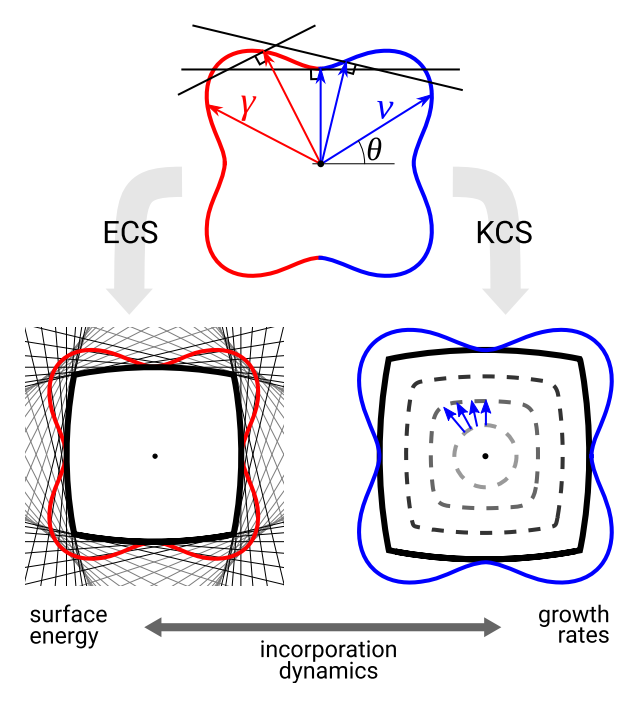
\includegraphics[width=0.6\textwidth]{ECS_vs_KCS_wulff_construction.png}
	\caption{Illustration of geometric similarity between Equilibrium Crystal Shape (ECS) driven by anisotropy in interface energy and Kinetic Crystal Shape (KCS) obtained by growth with growth rate having the same anisotropy. The top polar plot is the anisotropy function $h(\theta)$. Source:~\cite{Salvalaglio2015}.}
	\label{fig_ECS_vs_KCS_wulff_construction}
\end{figure}

It is not surprising to have the anisotropies in the interface energy and kinetic coefficients somehow related, because they both must derive from the state of the same interface. However, it is certainly interesting to realize that despite them being substantially different physical quantities, used for description of different processes, their anisotropy may manifest in similar ways. 

This was supported also by simulations of 2D growth of polycrystalline zeolite film using multi-phase field method~\cite{Wendler2011}. Reportedly, the same microstructures were obtained when assuming the same anisotropy in either interface energy or in the kinetic coefficient. 

While in crystal growth, the anisotropy in interface energy and kinetic coefficient may be interchangeable to some extent in terms of effect on the resulting shape (not on the shape evolution, though), there are necessarily processes where there is no overlap due to different nature of the quantities. For example, in nucleation, the nucleation barrier depends on the interface energy but does not depend on the kinetics. 

This interchangeability makes the experimental determination of these properties in-situ during deposition very complicated. However, in models of the deposition and in simulations, it is in fact necessary to distinguish the two quantities and then it is possible to distinguish also their impact of their anisotropy on the process. The mentioned phase-field method is one of methods capable to implement these quantities independently.

In the light of previous paragraphs, it is clear that while in some simulations it may not be a big problem to neglect anisotropy in either kinetic coefficient or interface energy as long as it is preserved in the other quantity. However, in the processes where these quantities are not interchangeable (e.g. anisotropic interface energy in nucleation barrier), neglecting the implications of anisotropy results in incomplete representation of the process.

%
%\section{Summary}
%This chapter contained fundamental information about the equilibrium stable shapes of particles with anisotropic interface energy, assuming absence of other driving forces which might affect their shape. Isolated particles as well as those on a plane were assessed in 2D.

%%%%%%%%%%%%%%%%%%%%%%%%%%%%%%%%%%%%%%%%%%%%%%%%%%
% Keep the following \cleardoublepage at the end of this file, 
% otherwise \includeonly includes empty pages.
\cleardoublepage

% vim: tw=70 nocindent expandtab foldmethod=marker foldmarker={{{}{,}{}}}
